\subsection{Object Transformers Model}

\begin{frame}[t,fragile]{Object Transformers Model}%{A Sub-title is optional}
\begin{center}
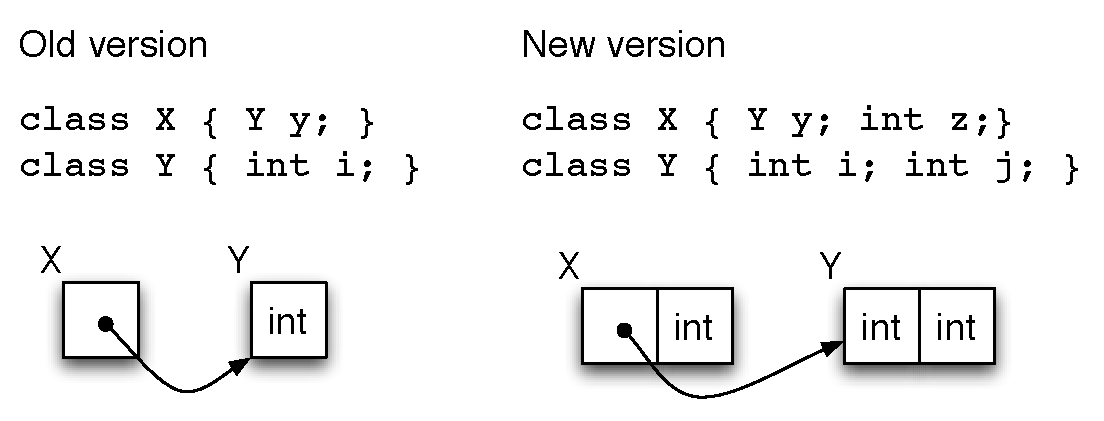
\includegraphics[scale=0.5]{images/object-transformers-model-example}
\end{center}
\begin{center}
% Transformers \\[1ex]
\begin{minipage}{0.4\textwidth}
\begin{lstlisting}[frame=single]
Transformer for X:
    to.y = from.y;
    to.z = 0;
Transformer for Y:
    to.i = from.i;
    to.j = 0;
\end{lstlisting}
\end{minipage}
\end{center}
\end{frame}

\begin{frame}[t,fragile]{Object Transformers Model}%{A Sub-title is optional}
\begin{center}
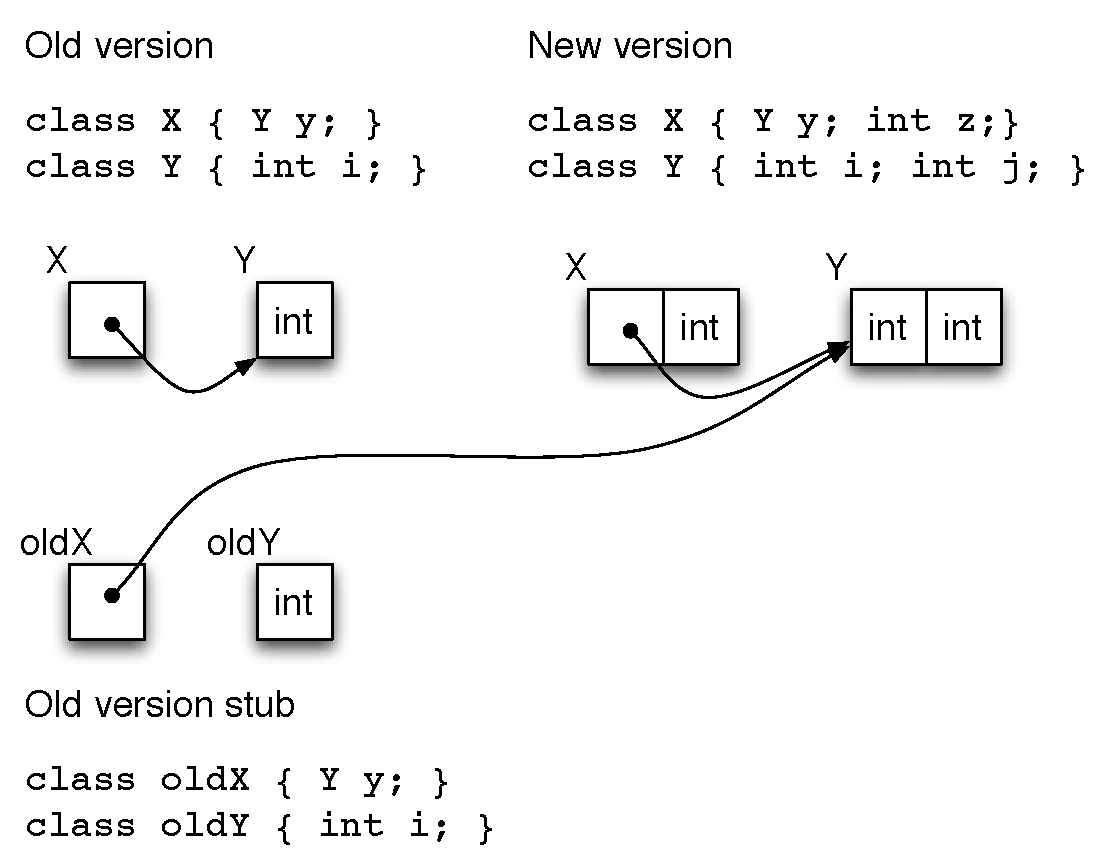
\includegraphics[scale=0.5]{images/object-transformers-model-example-1}
\end{center}
\end{frame}

\begin{frame}{Object Transformers Model}%{A Sub-title is optional}
\begin{itemize}
\item Simple to reason about
\item Transformers written in the source language
\item All references are to the newest version
\item Ensure that an object is transformed before reading its fields
\end{itemize}
\end{frame}
